\documentclass[../main.tex]{subfiles}

\begin{document}
\section{Theory}
\subsection{Logistic regression}
Logistic regression is a method for classifying a set of input variables \ensuremath{\boldsymbol{x}} to an output or class \ensuremath{y_i, i=1,2, \ldots,K} where $K$ is the number of classes. The review in this section is based on Hastie et al. \cite[ch.~4]{HastieTrevor2009EoSL},  and the reader is referred to this book for a more detailed explanation of topic. The prediction of output classes which the input variables belongs to is based on the design matrix \ensuremath{\boldsymbol{X}\in\mathbb{R}^{n\times p}} that contains $n$ samples that each carry $p$ features. We distinct between \textit{hard} and \textit{soft classification}, which determines the input variable to a class deterministically or the probability that a given variable belongs in a certain class. The logistic regression model is given on the form
 
\begin{align}
    \begin{split}
        \log\frac{p(G=1|X=x)}{p(C=K|X=x)}&=\beta_{10}+\beta_1^Tx \\
        \log\frac{p(G=2|X=x)}{p(C=K|X=x)}&=\beta_{20}+\beta_2^Tx \\
        &\vdots\\ 
        \log\frac{p(G=K-1|X=x)}{p(C=K|X=x)}&=\beta_{(K-1)0}+\beta_{K-1}^Tx.
    \end{split}
\end{align}

We consider the binary, two-class case with \ensuremath{y_i \in [0,1]}. The probability that a given input variable $x_i$ belongs in class $y_i$ is given by the Sigmoid-function (also called logistic function):
\begin{align}
    p(x) = \frac{e^x}{1+e^x}=\frac{1}{1+e^{-x}}.
\end{align}

A set of predictors, \ensuremath{\boldsymbol{\beta}}, which we want to estimate with our data then gives the probabilities 

\begin{align}
    p(y_i=1|x_i,\boldsymbol{\beta})=\frac{\exp\left(\boldsymbol{\beta}^Tx_i\right)}{1+\exp\left(\boldsymbol{\beta}^Tx_i\right)} \\
    p(y_i=0|x_i,\boldsymbol{\beta})=1-p(y_i=1|x_i,\boldsymbol{\beta}).
\end{align} We define the set of all possible outputs in our data set \ensuremath{\mathcal{D}(x_i,y_i)}. Further, we assume that all samples \ensuremath{\mathcal{D}(x_i,y_i)} are independent and identically distributed. Now we can approximate the total likelihood for all possible outputs of \ensuremath{\mathcal{D}} by the product of the individual probabilities \cite[p.~120]{HastieTrevor2009EoSL} of a specific output $y_i$:

\begin{align}
    P(\mathcal{D}|\boldsymbol{\beta}) = \prod_{i=1}^n[p(y_i=1|x_i\boldsymbol{\beta})]^{y_i}[1-p(y_i=1|x_i,\boldsymbol{\beta})]^{1-y_i}.
    \label{eq:likelihood}
\end{align} We want to maximize this probability by using the maximum likelihood estimator (MLE). By taking the logarithm of \cref{eq:likelihood}, we obtain the log-likelihood in \ensuremath{\boldsymbol{\beta}}

\begin{align}
    \log P(\mathcal{D}|\boldsymbol{\beta}) = \sum_{i=1}^n[y_i\log p(y_i=1|x_i\boldsymbol{\beta})+(1-y_i)\log(1-p(y_i=1|x_i,\boldsymbol{\beta}))].
    \label{eq:log-likelihood}
\end{align}

By reordering the logarithms and taking the negative of \cref{eq:log-likelihood}, we obtain the \textit{cross entropy}

\begin{align}
    \mathcal{C}(\boldsymbol{\beta})=-\sum_{i=1}^n\left[y_i\boldsymbol{\beta}^Tx_i-\log\left(1+\exp\left(\boldsymbol{\beta}^Tx_i\right)\right)\right].
    \label{eq:cross-entropy}
\end{align} The cross entropy is used as our cost function for logistic regression. We minimize the cross entropy, which is the same as maximizing the log-likelihood, and obtain

\begin{align}
    \frac{\partial\mathcal{C}(\boldsymbol{\beta})}{\partial\boldsymbol{\beta}}=-\sum_{i=1}^nx_i(y_i-p(y_i=1|x_i,\boldsymbol{\beta}))=0.
\end{align} The second derivative of this quantity is

\begin{align}
    \frac{\partial^2\mathcal{C}(\boldsymbol{\beta})}{\partial\boldsymbol{\beta}\partial\boldsymbol{\beta}^T}=\sum_{i=1}^nx_ix_i^Tp(y_i=1|x_i,\boldsymbol{\beta})(1-p(y_i=1|x_i,\boldsymbol{\beta})).
\end{align} These expressions can be written more compactly by defining the diagonal matrix \ensuremath{\boldsymbol{W}} with elements \ensuremath{p(y_i=1|x_i,\boldsymbol{\beta})(1-p(y_i=1|x_i,\boldsymbol{\beta}))}, \ensuremath{\boldsymbol{y}} as the vector with our $y_i$s values and \ensuremath{\boldsymbol{p}} as the vector of fitted probabilities. We can then express the first and second derivatives in matrix form

\begin{align}
    \frac{\partial\mathcal{C}(\boldsymbol{\beta})}{\partial\boldsymbol{\beta}}&=-\boldsymbol{X}^T(\boldsymbol{y}-\boldsymbol{p}) \\
    \frac{\partial^2\mathcal{C}(\boldsymbol{\beta})}{\partial\boldsymbol{\beta}\partial\boldsymbol{\beta}^T} &= \boldsymbol{X}^T\boldsymbol{W}\boldsymbol{X},
\end{align} also known as the Jacobian and Hessian matrices, respectively. We will use the stochastic gradient descent (SGD) (\cref{sec:sgd}) to find the optimal parameter \ensuremath{\boldsymbol{\beta}}. 


\subsection{Stochastic Gradient Descent}\label{sec:sgd}
\textit{Gradient descent} describes the process of finding a local minimum of a function (the cost function, in our case) by following the negative value of the gradient at each point, stepwise. \textit{Stochastic gradient descent} or SDG is a way of increasing the numerical efficiency of this process, by doing this process stochastically.

This involves randomly dividing the training data into a given number of \textit{mini batches}. For each mini batch, the gradient is found by averaging the gradient value each mini batch sample has. Then the weights and biases are updated (take a step down the "slope") and the process is repeated for the rest of the mini batches. The updating done at each mini batch is expressed mathematically as

\begin{align*}
    w&\rightarrow w' = w - \frac{\eta}{m}\sum_i^m \nabla C_{i,w} \\
    b&\rightarrow b' = b - \frac{\eta}{m}\sum_i^m \nabla C_{i,b},
\end{align*}

where $m$ is the number of datapoints in the mini batches and $\nabla C_i$ is the gradient at each individual data point. After exhausting all the training data, we have finished a so-called \textit{epoch}, of which we can perform as many as necessary.

\subsection{Error metrics/Quality of models}
We measure the performance of the different models used in this work. For classification, we measure how accurate the predictions given by the model are by the so called accuracy score. The accuracy score is given by

\begin{align}
    \text{accuracy}=\frac{1}{n}\sum_{i=0}^nI(t_i=y_i),
    \label{eq:accuracy-score}
\end{align} where $n$ is the number of samples, $t_i$ represents the target output and $I$ is the indicator function, which returns 1 if \ensuremath{y_i=t_i} and 0 otherwise. 

%For regression, MSE and R2 score, refer reader to project1


\subsection{Franke's function}
Franke’s function is a function which is often used to test different regression and interpolation methods. The function has two Gaussian peaks of differing heights, and a smaller dip \cite{FrankeRichard1979}. Therefore the dataset is perfect for studying how a neural network can be used to predict the well known function. It's expression is

\begin{align}
\begin{split}
  f(x,y) &= \frac{3}{4}\exp{\left(-\frac{(9x-2)^2}{4} - \frac{(9y-2)^2}{4}\right)}+\frac{3}{4}\exp{\left(-\frac{(9x+1)^2}{49}- \frac{(9y+1)}{10}\right)} \\
  &+\frac{1}{2}\exp{\left(-\frac{(9x-7)^2}{4} - \frac{(9y-3)^2}{4}\right)} -\frac{1}{5}\exp{\left(-(9x-4)^2 - (9y-7)^2\right) }.
\end{split}
  \label{eq:franke-func}
\end{align}

In the defined interval $x,y\in[0,1]$. For more information about Franke's function see \cite{project2}. An illustration of Franke's function can be seen in figure \ref{fig:frankesplot}

\begin{figure}[H]
  \centering
  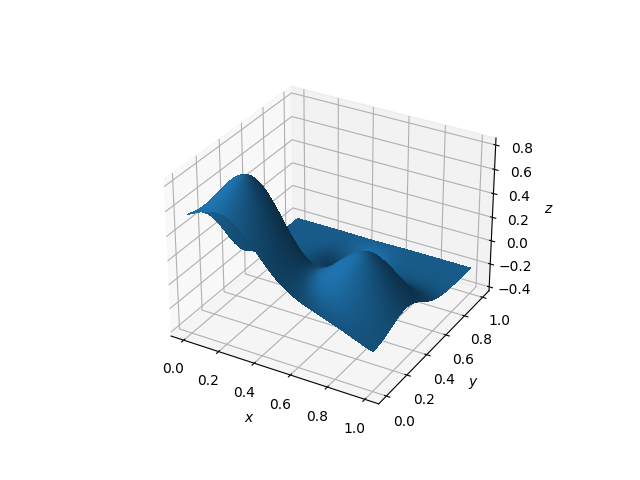
\includegraphics[trim=2.4cm 1cm 1.4cm 1cm, clip,width = 3in]{../assets/actual_franke_plot.png}
  \caption{Shape of Franke's function which will be used as a interpolating goal}
  \label{fig:frankesplot}
\end{figure}


\end{document}